
\subsubsubsection{Laser positioning system}
\label{sec:calib-laser-pos}
\paragraph{Physics Motivation}

While the direction of the laser beam will be very well known based on the reading from the encoders on the laser beam steering mechanism,  residual uncertainty or unpredictable shift in the pointing direction will remain. Having in mind long length of the ionization track of more than 15\,m, even a small offset in the pointing direction can lead to vastly different ionization track location, especially close to the end of
the track. Such inaccuracies will directly impact the ability to precisely calibrate any variations in the \efield.

\paragraph{Design}

Laser positioning system (LPS) is designed to address the problem of precise and accurate knowledge of the laser track coordinates. %University of Hawaii group has 
Such a system (consisting of 1$\times$3) array was built for the miniCAPTAIN experiment and installed version is visible in the photo of the miniCAPTAIN TPC Fig.~\ref{fig:miniCAPTAIN}.  
\begin{figure}[htb!] 
\centering 
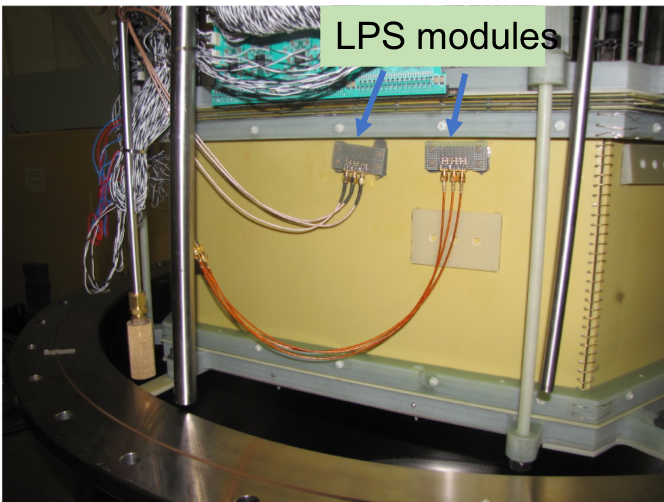
\includegraphics[width=0.6\linewidth]{LPS_miniCAPTAINlabeled.png} 
\caption{Photo of the miniCAPTAIN TPC with two LPS modules glued on the outside, in order to detect laser beam spot location via fluorescence of the TPC FR4 wall when illuminated by the laser beam.}
\label{fig:miniCAPTAIN} 
\end{figure}
LPS consists of groups of 9 pin diodes, operating in passive, photovoltaic mode. These are GaP diodes whose sensitivity range extends down to 200\,nm wavelength --- thus detecting 266\,nm light is straightforward. Fig.~\ref{fig:LPS1} and Fig.~\ref{fig:LPS2}  show signal detected at room and cryogenic
temperatures. PIN diode was illuminated by the 266\,nm light from the NdYag
laser in the lab 
%(in the lab at University of Hawaii) 
set at lowest possible setting for minimal power. Pin diode pads receive light via optical fiber bundles that are mounted on the opposite side from the laser injection points to eliminate issues with field cage interference. Drawings of one such group of pin diodes is shown in Figs.~\ref{fig:pin1} and Fig.~\ref{fig:pin2}. With the group of 9 photodiodes, one cannot only detect the beam but also crudely characterize its profile, giving a more precise location of the central beam pulse axis.


%\begin{figure}[htb!] 
%\begin{minipage}[b]{0.47\textwidth}
%\centering 
%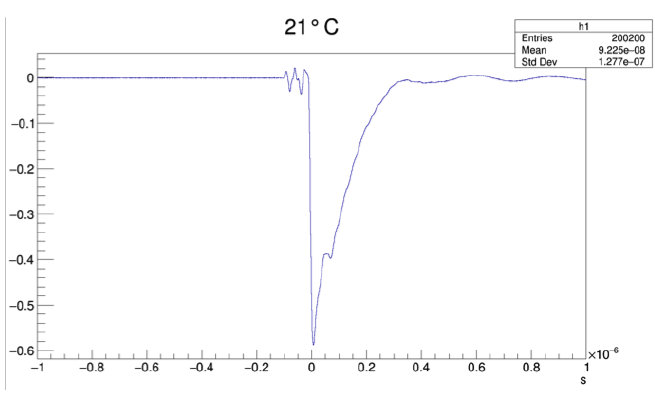
\includegraphics[width=0.95\linewidth]{GaP_diode_room_temp.png} 
%\caption{Signal from the GaP pin diode. The signal was a result of illumination of the PIN diode face with a 266\,nm laser at room temperature.}
%\label{fig:LPS1} 
%\end{figure}
%\end{minipage}
%\hfill
%\begin{minipage}[b]{0.47\textwidth}
%\begin{figure}[htb!] 
%\centering 
%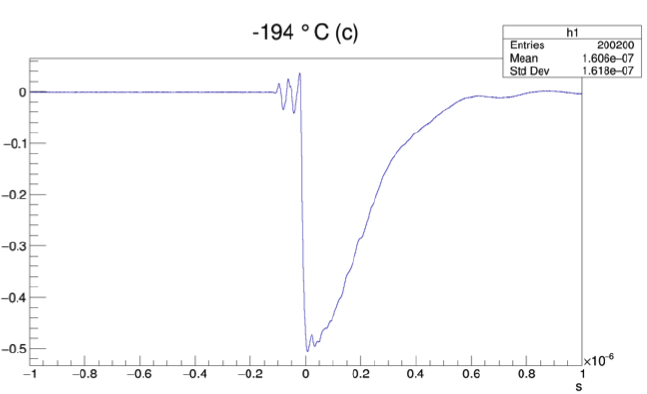
\includegraphics[width=0.95\linewidth]{GaP_diode_cryo_temp.png} 
%\caption{Signal from the GaP pin diode. The signal was result of illumination of the PIN diode face with a 266\,nm laser at cryogenic temperature.}
%\label{fig:LPS2} 
%\end{minipage}
%\hfill
%\end{figure} 


\begin{figure}[htb!] 
\begin{minipage}[b]{0.47\textwidth}
\centering 
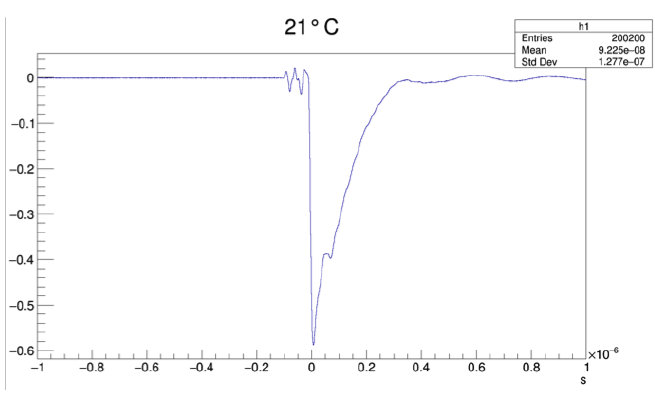
\includegraphics[width=1.0\linewidth]{GaP_diode_room_temp.png} 
\caption{Signal from the GaP pin diode. The signal was a result of illumination of the PIN diode face with a 266\,nm laser at room temperature.}
\label{fig:LPS1} 
\end{minipage}
\hfill
\begin{minipage}[b]{0.47\textwidth}
\centering 
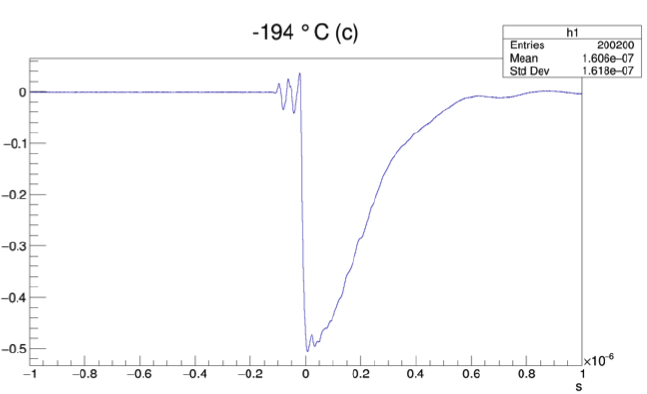
\includegraphics[width=1.0\linewidth]{GaP_diode_cryo_temp.png} 
\caption{Signal from the GaP pin diode. The signal was result of illumination of the PIN diode face with a 266\,nm laser at cryogenic temperature.}
\label{fig:LPS2} 
\end{minipage}
\hfill
\end{figure} 

\begin{figure}[htb!] 
\begin{minipage}[b]{0.4\textwidth}
\centering 
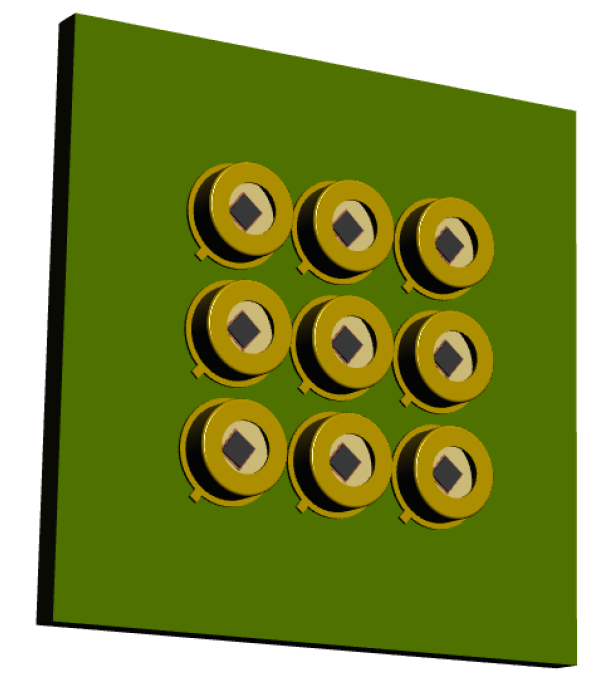
\includegraphics[width=0.95\linewidth]{GaP_assembly.png} 
\caption{LPS cluster that is mounted on the opposite wall from the laser periscope to detect and accurately determine the end point of the laser beam.}
\label{fig:pin1} 
\end{minipage}
\hfill
\begin{minipage}[b]{0.47\textwidth}
\centering 
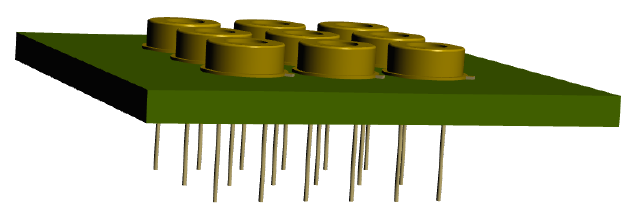
\includegraphics[width=0.95\linewidth]{GaP_assembly_profile.png} 
\caption{Profile of the LPS group mounted on the PCB. GaP diodes come with pins that utilize twisted pair to transport the signal.}
\label{fig:pin2} 
\end{minipage}
\hfill
\end{figure} 

There will be one LPS pad per laser. Laser would always send the first pulse in the direction of the LPS before proceeding into a calibration sequence.
 The electronics used to collect
signals from the LPS will be provided by the slow control group.

\paragraph{Possible measurements}
The utilization of the fiber bundle to deliver the 266\,nm photons to LPS needs to be verified in the lab. Lab measurements are currently underway to measure light attenuation in the fiber bundles (that go to the GaP diodes) as a function of fiber diameter and length. Further optimization of the LPS assembly to reduce electronic noise and cross-talk is required, among other things. Another important aspect is durability of the system that will require extensive running in the cryogenic conditions with  a large number of cool-downs to validate GaP for extended use in DUNE. Finally, alternatives to GaP such as SiPMs are under consideration. While SiPMs require power, their sensitivity to single photons makes them a desirable candidate for low light signals. 
